\begin{frame}{Limitações do Bench4Q para analise não-estacionária}
	\begin{itemize}
		%\item Projetado para avaliação de desempenho tradicional;
		\item Não possui instrumentação para modulação da carga de trabalho;
		\begin{itemize}
			\item O número e configurações dos agentes são definidos uma  só vez antes de cada experimento;			 
		\end{itemize}
		\item O objetivo deste trabalho é estender a carga de trabalho do \textit{benchmark} Bench4Q para que seja possível estimular o sistema a apresentar a sua dinâmica, e assim possibilitando a analise transiente do sistema, incorporando-se o modulo \textit{Demand} da arquitetura conceitual MEDC.
	\end{itemize}
	
	
	
	\note{Explicar que o Bench4q é um sistema em lote (bach) que coloca o SUT em condição estacionária. Explicar que não possui instrumentação para modulação de demanda ou capacidade.  Explicar que não há divisão de responsabilidade para modelagem da dinâmica.}
\end{frame}

\begin{frame}{Extensão do Bench4Q}
	\begin{itemize}
		\item Exemplificar por meio da extensão do Bench4Q para atender os requisitos MEDC;
		\item O resultado final é avaliado por meio de exemplos de uso do \textit{benchmark} estendido;
		\item Foi possível expor:
		\begin{itemize}
			\item A dinâmica do sistema investigado, evidenciando:
			\begin{itemize}
				\item A utilidade da avaliação de desempenho não estacionária;
				\item A capacidade do \textit{benchmark} estendido via MEDC em atender aos requisitos.
			\end{itemize} 
		\end{itemize} 
	\end{itemize}
\end{frame}


\begin{frame}{Proposta}
	\begin{itemize}
		
		\item \textbf{Tempo de início:} instante em que a carga modulada inicia a geração de requisições;
		
		\item \textbf{Tempo de planejamento de carga:} Um período de tempo em que a carga de trabalho é modulada, caracterizando a mudança do comportamento das requisições de maneira programada;
		
		\item \textbf{Tempo de interrupções:} Período de interrupções/pausa após o \textit{Tempo de planejamento de carga};
		
		\item \textbf{Quantidade de clientes na modulação:} reservar uma quantidade de clientes EBs, que estão com dedicação exclusiva para a modulação da carga.
	\end{itemize}	
\end{frame}


\begin{frame}{Possibilidade de cargas moduláveis pela extensão}
	\begin{itemize}
		\item \cite{Hellerstein2004}, apresentam algumas funções, de perturbação, capazes de excitar o sistema a apresentar a sua dinâmica por exemplo: pulso, degrau, etc.
	\end{itemize}
	
	\begin{columns}
		\column{0.4\textwidth}
		\begin{minipage}[c][0.4\textheight][c]{\linewidth}
			\centering
			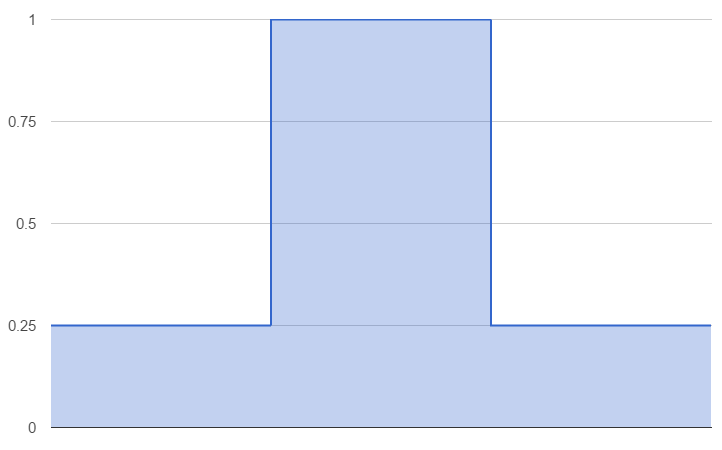
\includegraphics[width=0.84\linewidth]{../monograph/images/carga-sintetica1.png}
			\label{fig:degrau-positivo}
		\end{minipage}
		\begin{minipage}[c][0.4\textheight][t]{\linewidth}
			\centering
			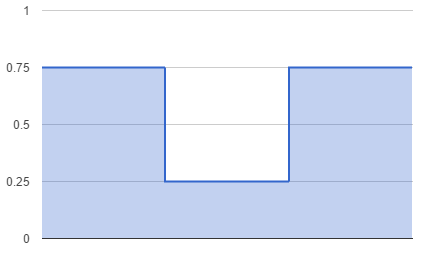
\includegraphics[width=0.84\linewidth]{../monograph/images/carga-sintetica2.png}
			\label{fig:degrau-negativo}
		\end{minipage}
		\column{0.4\textwidth}
		\begin{minipage}[c][0.4\textheight][c]{\linewidth}
			\begin{enumerate}
				\item Pulso positivo,
				\item Pulso negativo,
				\item Onda quadrada;
			\end{enumerate}
		\end{minipage}
		\begin{minipage}[c][0.4\textheight][t]{\linewidth}
			\centering
			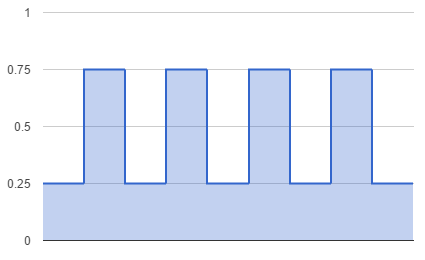
\includegraphics[width=0.84\linewidth]{../monograph/images/carga-sintetica3.png}
			\label{fig:onda-gradrada}
		\end{minipage}
	\end{columns}
	
\end{frame}

\begin{frame}{Implementação da carga de trabalho}
	\begin{figure}[htb]
		\centering
		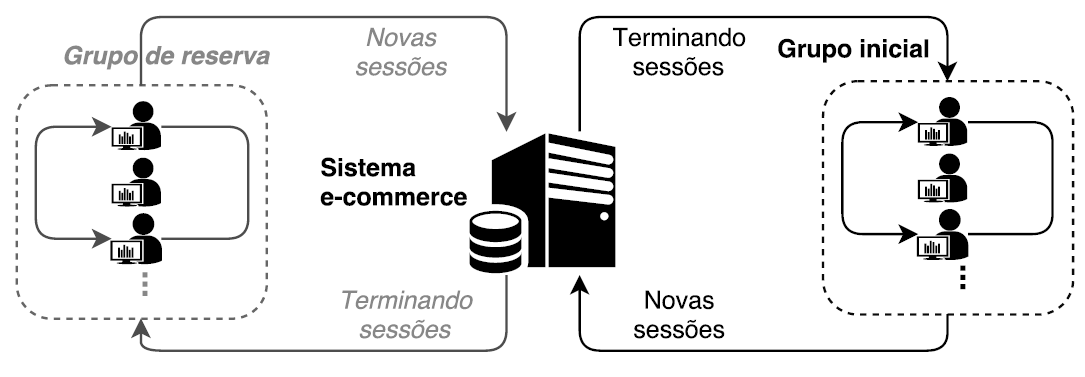
\includegraphics[scale=0.4]{images/operacaoes_dentro_sessao.png}	
		\caption{Modulação da carga de trabalho \cite{Edwin2015}}
	\end{figure}
\end{frame}
